%% Gas-star segregation and the resilience of King-family clusters to
%% gas expulsion: a semi-analytic study.  B. Shukirgaliyev.
%% Figures and data tables are reproduced by the scripts under code/;
%% see code/REPRODUCTION_GUIDE.md and docs/figure_data_map.csv.
\documentclass{aa}

\usepackage{graphicx}
\usepackage{txfonts}
\usepackage{amsmath}
\usepackage[hidelinks]{hyperref}
\usepackage[flushleft]{threeparttable}
\usepackage{placeins}

\newcommand{\esfe}{e{\rm SFE}}
\newcommand{\sfe}{{\rm SFE}}
\newcommand{\Msun}{{\rm M}_\odot}
\newcommand{\rhalf}{r_{\rm h}}
\newcommand{\rtid}{r_{\rm t}}
\newcommand{\rsf}{r_{\rm SF}}
\newcommand{\tsf}{t_{\rm SF}}
\newcommand{\tff}{t_{\rm ff}}
\newcommand{\effE}{\varepsilon_{\rm ff}}

% Float placement. The aa class allows up to six floats per page, four of
% them at the top, which lets figures pile up. Cap it at two per page (one
% for full-width floats); a few figures carry [b] so they fall to the next
% page rather than crowd their neighbours.
\AtBeginDocument{%
  \setcounter{topnumber}{2}%
  \setcounter{bottomnumber}{1}%
  \setcounter{totalnumber}{2}%
  \setcounter{dbltopnumber}{1}%
}
\renewcommand*\topfraction{0.85}
\renewcommand*\bottomfraction{0.55}
\renewcommand*\textfraction{0.12}
\renewcommand*\dbltopfraction{0.85}
\renewcommand*\floatpagefraction{0.60}
\renewcommand*\dblfloatpagefraction{0.60}

\begin{document}

\title{Gas--star segregation and the resilience of King-family
clusters to gas expulsion: a semi-analytic study}
\titlerunning{Gas--star segregation and King-cluster resilience}
\authorrunning{B. Shukirgaliyev}
\author{B.~Shukirgaliyev\inst{1,2,3}\thanks{ORCID:
0000-0002-4601-7065}}

\institute{Department of Physics, Nazarbayev University, 53 Kabanbay Batyr ave., Astana, Kazakhstan\\
           \email{bekdaulet.shukirgaliyev@nu.edu.kz}
      \and Energetic Cosmos Laboratory, Nazarbayev University, 53 Kabanbay Batyr ave., Astana, Kazakhstan
      \and Fesenkov Astrophysical Institute, 23 Observatory str., Almaty, Kazakhstan
      \and
      K. Zhubanov Aktobe Regional University, 263 Zhubanov str., Aktobe, Kazakhstan
      }

\date{Received ; accepted }

\abstract
% context
{Star clusters survive instantaneous gas expulsion more easily when the
star formation efficiency (SFE) is centrally peaked, since the stars are
then born more concentrated than the gas they must unbind from. King
models have been used in this setting before, but with a residual gas
component of free shape and normalization. The case in which the gas
instead follows from the star formation itself, leaving both components
truncated and the global SFE unambiguous, has not been mapped, although
the King family is the one adopted by upcoming $N$-body campaigns.}
% aims
{We quantify how the survivability of an embedded King-model cluster
depends on the concentration parameter $W_0$, identify the physical
mechanism that controls it, and provide calibrated initial-condition
predictions for direct $N$-body simulations.}
% methods
{Assuming a constant SFE per free-fall time, we derive in closed form
(up to quadratures) the residual-gas profile for King models with
$W_0=0.5$--$20$ and compute the post-expulsion virial ratio, calibrated
against the effective SFEs inferred at the published Plummer and Dehnen
$N$-body thresholds. Independently, we obtain the bound mass fraction
from a frozen stellar distribution function via an analytic Eddington
inversion in the total star--gas potential, cross-checked against Monte
Carlo realizations drawn from the same function.}
% results
{The virial criterion yields an SFE threshold that is non-monotonic in
$W_0$, falling to $\simeq0.11$ near $W_0\simeq8.8$ for the reference
choice $\esfe_{\rm surv}=1/3$. The dependence reduces exactly to one
dimensionless parameter, the normalized star--gas cross energy per unit
gas mass, whose minimum lies near the maximum of the King structural
ratio $\rtid/\rhalf$, where gas--star segregation is greatest. The
frozen-DF analysis reproduces the same trend independently and predicts
that concentrated models keep a self-bound central seed down to global
SFEs of a few per cent. The survival value of the effective SFE is not
universal across density profiles.}
% conclusions
{Clusters born with intermediate King concentrations
($W_0\approx8$--$9$) are the most resilient to instantaneous gas
expulsion. The predicted ordering with $W_0$ -- rather than any single
absolute threshold -- is the sharp, falsifiable result that the
$N$-body campaign of Paper~I will test.}
\keywords{galaxies: star clusters: general -- methods: analytical --
          methods: numerical -- stars: formation --
          stars: kinematics and dynamics}

\maketitle

%-------------------------------------------------------------------
\section{Introduction}
%-------------------------------------------------------------------

The response of a young star cluster to the loss of its residual
star-forming gas is a long-standing problem of cluster dynamics
\citep{Hills1980,Lada2003,BoilyKroupa2003a,BaumgardtKroupa2007}. When
the stars and the gas share the same density profile, the classical
instantaneous-loss virial argument requires a global star formation
efficiency of $\sfe>0.5$ for the remnant to stay bound, while $N$-body
experiments, in which the cluster re-virializes and keeps a bound core,
lower this to $\sfe\simeq0.33$
\citep{BoilyKroupa2003a,BoilyKroupa2003b,BaumgardtKroupa2007}. The
star formation efficiencies inferred for embedded clusters are typically
well below this value, so the identical-profile picture predicts near
universal dissolution -- in tension with the observed population of
bound clusters.

The resolution, recognised well before the present framework, is that a
stellar component \emph{more centrally concentrated than the gas}
survives expulsion far more readily. \citet{Adams2000} built
semi-analytic models in which the stars follow a lowered-isothermal
(King) distribution function in the combined star--gas potential -- the
construction we adopt here -- with an ad hoc untruncated isothermal gas
halo of free amplitude, and found substantial survival well below the
classical threshold; $N$-body surveys with static gas potentials
\citep{Adams2006,ProszkowAdams2009} confirmed the picture. What these
models left unspecified is the \emph{origin} of the gas--star density
contrast: the gas profile and its normalization were free parameters
rather than consequences of the star formation process.

\citet{Parmentier2013} closed that gap. Star formation at a constant
efficiency per free-fall time, $\effE$ \citep{KrumholzMcKee2005}, inside
a centrally concentrated clump necessarily leaves a stellar component
\emph{steeper} than the residual gas: the local SFE is centrally peaked.
In \citet[hereafter S17]{Shukirgaliyev2017} we showed with direct
$N$-body models that Plummer clusters formed this way survive
instantaneous gas expulsion down to $\sfe\simeq0.15$, an effective SFE
(Sect.~\ref{sec:esfe}) of $\simeq0.32$, insensitively to the Galactic
tide \citep{Shukirgaliyev2019}. In
\citet[hereafter S21]{Shukirgaliyev2021} we extended this to
\citet{Dehnen1993} profiles, where survivability improves with a
shallower outer slope and a steeper cusp: the lowest surviving efficiency
sampled, $\sfe_{\rm J}=0.01$ within the Jacobi radius, was reached by the
$\gamma=2$ and $2.5$ models.

Fully coupled (magneto)hydrodynamical$+$$N$-body simulations of cluster
formation with star-by-star feedback have matured rapidly
\citep[e.g.][]{Wall2019,Lahen2020,Grudic2021,Hirai2021,Fujii2021c,
Dinnbier2020}. They constrain two ingredients of the present framework:
feedback-driven gas expulsion proceeds on roughly the free-fall time of
the star-forming clump \citep{Li2019}, dynamically close to the
instantaneous limit \citep{BaumgardtKroupa2007}, and \citet{Fujii2021c}
find that star-by-star cluster formation with feedback yields cluster
masses and radii matching a comparable calculation that assumed
instantaneous star formation and gas expulsion \citep{FujiiPZ2016},
concluding that the simplified treatment suffices for the cluster mass
function and for the dynamical evolution after gas expulsion. What such
simulations cannot yet deliver is statistics over initial-condition
families. In our own models of this channel the wall-clock cost per
realization grew from about a week at the coarsest refinement to seven
months at the finest, so ensembles of ten realizations were affordable
only at the coarsest level, and the outcome is highly sensitive to the
stochastic details of massive-star feedback -- when the first very
massive star forms, its mass and position, and the adopted jet model --
so that identical initial conditions yield markedly different cluster
structures \citep{Assilkhan2026,AssilkhanJets2026,Akhmetali2026}.
Statistics over realizations are therefore mandatory rather than
optional, and mapping survivability across a family of initial structures
requires tens of runs per parameter combination. The semi-analytic
framework developed here is complementary to the coupled runs: they
calibrate the sub-grid ingredients ($\effE$, the expulsion timescale),
while it maps the parameter space with the statistics the problem
demands.

The S17 and S21 initial conditions share two limitations. First, a
Plummer stellar profile formed at constant $\effE$ leaves a residual gas
profile steeper than the dust-continuum profiles of observed young
clumps. Second, and more basic, the Plummer and Dehnen profiles are
spatially infinite, so the ``global'' SFE depends on the aperture within
which it is measured -- S17's value was effectively aperture-limited, and
S21 had to quote the SFE within the Jacobi radius and convert. Real
embedded clusters, moreover, are routinely described by King models
\citep{King1966}, and the forthcoming $N$-body campaign (Paper~I, in
prep.) adopts them.

This paper therefore builds a King-family initial-condition set. Both the
stars and the residual gas are finite -- truncated together at the
tidal radius -- so the global SFE is a single unambiguous number, and the
concentration $W_0$ becomes a free axis along which to map
survivability. We work out, fully analytically up to quadratures, the
structure and post-expulsion virial state of these models; check the
virial machinery against the published S17/S21 thresholds; add a fully
independent distribution-function estimate of the bound fraction; and
derive the survivability predictions Paper~I will test.

The paper is organized as follows. Section~\ref{sec:ics} constructs the
King-family initial conditions and their local-SFE structure.
Section~\ref{sec:virial} develops the post-expulsion virial state,
reduces the survival condition to a single dimensionless parameter,
compares the King predictions with the published families, and gives the
threshold curve and its mechanism. Section~\ref{sec:df} computes the
bound fraction from the frozen distribution function and verifies it with
Monte Carlo realizations. Section~\ref{sec:truncation} introduces the
free-fall-time truncation criterion. We discuss the implications in
Sect.~\ref{sec:discussion} and conclude in Sect.~\ref{sec:conclusions}.
The appendix documents the numerical verification of every quadrature
and inversion used.

A note on terminology. Every SFE at which a cluster is deemed to survive
in this paper is the output of a specific static criterion, not a
dynamical result, and we name it accordingly. Two of these live in
global-SFE space and are functions of $W_0$: $\sfe_{\rm vir}$, the
\emph{virial threshold}, is the global SFE at which the post-expulsion
virial ratio reaches an adopted survival value of the effective SFE,
$\esfe_{\rm surv}$; and $\sfe_{\rm DF}$, the \emph{frozen-DF threshold},
is the global SFE at which the bound fraction of the frozen distribution
function falls below $F_{\rm b}=0.02$. The survival value
$\esfe_{\rm surv}$ is a quantity of a different kind: a single adopted
number in effective-SFE space (we take the classical $1/3$ throughout),
the \emph{input} to the virial criterion, whereas $\sfe_{\rm vir}$ is its
\emph{output} and runs from $0.225$ to $0.106$ across the $W_0=3$--$9$
grid of Paper~I.

A convention for the SFE itself is needed because the families compared
here are not all finite. For the King models both components are
truncated at $\rtid$, so the global SFE
$\sfe=M_\star/(M_\star+M_{\rm g})$ is unambiguous. The published Plummer
and Dehnen models are spatially infinite, and we follow S17 and S21 in
measuring their SFE within ten scale radii, $\sfe_{10}$. Throughout the
paper we write simply $\sfe$, meaning the total value for King models and
$\sfe_{10}$ for the published families; axes and tables are labelled
accordingly and the distinction is flagged again only where the two are
plotted together.

We reserve the term \emph{critical SFE}, $\sfe_{\rm crit}$, for the
dynamical threshold of a live cluster as measured in direct $N$-body
simulations. It is not computed anywhere in this paper:
$\sfe_{\rm vir}$ and $\sfe_{\rm DF}$ are static estimates of it, and the
$N$-body campaign of Paper~I is what will measure it. That measurement
will itself be a prediction rather than a fact about real clusters,
inheriting the idealizations of instantaneous expulsion and of gas that
is removed rather than evolved; but it is the closest proxy available,
and it is the number the estimates made here are to be judged against.

%-------------------------------------------------------------------
\section{King-family initial conditions}
\label{sec:ics}
%-------------------------------------------------------------------

\subsection{Stellar King profile}
\label{sec:stars}

The stellar cluster immediately before gas expulsion is a King model of
concentration $W_0$ \citep{King1966}. The construction of stars in
virial equilibrium within the total star--gas potential follows
\citet{Adams2000}; the essential difference is that here the gas profile
is not free but is fixed by the star formation physics
(Sect.~\ref{sec:gas}), which ties the density contrast, the truncation,
and the global SFE together. Our $W_0$ parametrizes the \emph{stellar}
King profile, whereas the well depth $\psi_0$ of \citet{Adams2000} is
defined in the total potential.

We present the structural figures in units $G=M_\star=r_{\rm h}=1$, with
$M_\star$ the total stellar mass and $r_{\rm h}$ the stellar half-mass
radius. This matches the companion $N$-body campaign, which fixes the
tidal filling factor $\lambda\equiv r_{\rm h}/R_{\rm J}$ across $W_0$ --
i.e.\ it equates half-mass radii, not tidal radii -- so a half-mass-radius
normalisation is the one in which the models are actually compared. (S17
and S21 used core-radius and scale-length units respectively; the
underlying King solution is computed in $G=M_\star=r_0=1$ with $r_0$ the
King scale radius, then rescaled.) Every SFE and $\esfe$ quantity below is
dimensionless and invariant under the choice of length unit
(Sect.~\ref{sec:gas}). For reference, the models used in the campaign
have
$(W_0,\,c\equiv\log_{10}\rtid/r_0,\,r_{\rm t}/r_{\rm h})=
(3,\,0.672,\,3.73)$, $(6,\,1.255,\,6.80)$, and $(9,\,2.119,\,8.54)$.

\subsection{Residual gas}
\label{sec:gas}

Star formation proceeds for a duration $\tsf$ at a constant efficiency
per free-fall time $\effE$ \citep{KrumholzMcKee2005,Parmentier2013}. We
adopt $\effE=0.01$ as a fiducial value motivated by measurements on
molecular-cloud and larger scales
\citep{KrumholzMcKeeBlandHawthorn2019,Utomo2018,Pokhrel2021} -- reported
values span roughly an order of magnitude, and \citet{Parmentier2013}
themselves normalized at $\effE\simeq0.1$ -- and explore the sensitivity
in Sect.~\ref{sec:truncation}, which also shows that every untruncated
result below is exactly independent of this choice. As shown below, this
choice affects only the free-fall-time truncation of
Sect.~\ref{sec:truncation}; every other result is exactly independent of
$\effE$. Defining
\begin{equation}
  k \equiv \sqrt{\frac{8}{3\pi}}\, \effE\, \tsf ,
  \label{eq:k}
\end{equation}
the local \citet{Parmentier2013} relation between the stellar density
$\rho_\star$ and the residual gas density $\rho_{\rm g}$ inverts in
closed form. With $\alpha\equiv k^4\rho_\star^2$ and
\begin{align}
  K_0 &= \left[\alpha^3+36\alpha^2+216\alpha
        +24\alpha\sqrt{3(\alpha+27)}\right]^{1/3}, \nonumber\\
  K_1 &= \sqrt{\frac{\alpha^2+\alpha(K_0+24)+K_0(K_0+12)}{12\,k^4K_0}},
        \nonumber\\
  K_2 &= \frac{(\alpha-K_0+24)(K_0-\alpha)}{3\,k^4K_0},
\end{align}
the gas density is
\begin{equation}
  \rho_{\rm g} \;=\; \frac{1}{k^2} \;-\; \frac{\rho_\star}{2}
  \;-\; \frac{1}{2}\sqrt{K_2+\frac{8}{k^6 K_1}} \;+\; K_1 .
  \label{eq:gas}
\end{equation}
Equation~(\ref{eq:gas}) has two informative limits. Where the stellar
density is high the gas saturates at a constant plateau,
$\rho_{\rm g}\rightarrow1/k^2$, and the local SFE
$\rho_\star/(\rho_\star+\rho_{\rm g})\rightarrow1$: the cluster centre is
gas-poor. Where the stellar density is low,
$\rho_{\rm g}\propto\rho_\star^{2/3}$: the gas is shallower than the
stars and dominates the outskirts. Because
$\rho_{\rm g}\rightarrow0$ as $\rho_\star\rightarrow0$, the gas of a King
cluster is truncated together with the stars at the King radius
$\rtid$; the gas mass, and hence the global SFE
$\sfe=M_\star/(M_\star+M_{\rm g})$, are finite and fully set by
$(W_0,\tsf)$.

A simultaneous rescaling $\rho\rightarrow c\rho$,
$k\rightarrow c^{-1/2}k$ leaves Eq.~(\ref{eq:gas}) form-invariant and
merely relabels $\tsf$; every dimensionless result below is therefore
independent of the unit convention. For the same reason $\effE$ and
$\tsf$ enter only through $k$: every untruncated result of this paper is
\emph{exactly} independent of the adopted $\effE$
(Sect.~\ref{sec:truncation}).

\subsection{Structure of embedded King clusters}
\label{sec:structure}

Figure~\ref{fig:structure} shows the stellar and gas density profiles of
the $W_0=3,6,9$ models at a fixed global $\sfe=0.17$ (panel a) and the
corresponding local SFE profiles for $W_0=0.5$--$20$ (panel b). The behaviour anticipated in Sect.~\ref{sec:gas} is
apparent: the local SFE approaches unity at the centre, falls through
the global value near the half-mass radius, and the gas -- everywhere
shallower than the stars -- is truncated with them at $\rtid$, which for
these concentrations lies at $r_{\rm t}/r_{\rm h}\simeq4$--$9$. Both
components being finite, the global SFE
$\sfe=M_\star/(M_\star+M_{\rm g})$ is a single well-defined number, not
an aperture-dependent one. The mapping between $\tsf$ and the global SFE
for the whole family is given in Fig.~\ref{fig:sfetsf}.

\begin{figure}[t]
\centering
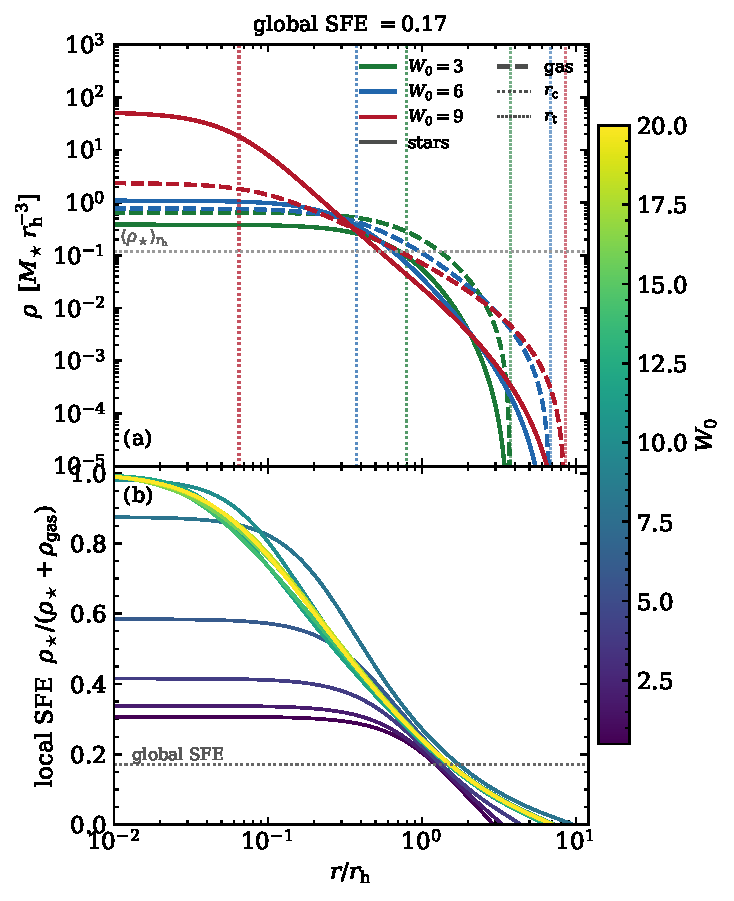
\includegraphics[width=\hsize]{figures/fig1_structure.pdf}
\caption{King structure at a global $\sfe=0.17$, in units $G=M_\star=r_{\rm h}=1$.
\emph{(a)} Stellar (solid) and residual gas (dashed) densities for
$W_0=3,6,9$; coloured verticals mark $r_0$ (dotted) and $\rtid$ (fine
dotted), the grey line the mean stellar density within $r_{\rm h}$,
$3/(8\pi)$. \emph{(b)} Local SFE $\rho_\star/(\rho_\star+\rho_{\rm g})$
for $W_0=0.5$--$20$; dotted line, the global value.
See Sect.~\ref{sec:structure}.}
\label{fig:structure}
\end{figure}

\begin{figure}[b]
\centering
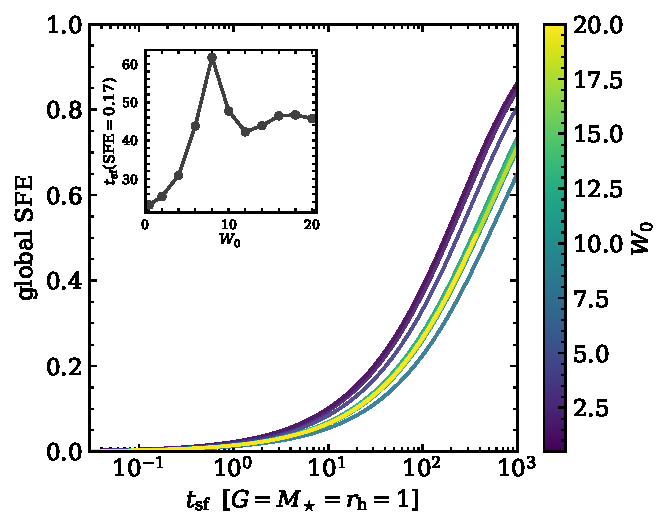
\includegraphics[width=\hsize]{figures/fig3_sfe_vs_tsf_rh_units.pdf}
\caption{Global SFE against the star formation duration for the King
family, with time in units $G=M_\star=r_{\rm h}=1$ and the fiducial
$\effE=0.01$. The curves lie within a factor of $\simeq2.7$ of one
another across $W_0=0.5$--$20$ (inset): at $\effE=0.01$ reaching
$\sfe=0.17$ takes $\tsf\simeq23$ ($W_0=0.5$) to $\simeq63$ ($W_0=8$),
i.e.\ $\simeq15$--$40$ free-fall times of the half-mass region
($\tff(r_{\rm h})\simeq1.6$ in these units) -- the low efficiency, not
the geometry, sets the absolute scale.}
\label{fig:sfetsf}
\end{figure}

%-------------------------------------------------------------------
\section{Post-expulsion virial state and the SFE threshold}
\label{sec:virial}
%-------------------------------------------------------------------

\subsection{Effective SFE}
\label{sec:esfe}

The stars are taken to be in virial equilibrium within the total
(stars $+$ gas) potential at the instant of gas expulsion (S17). The
scalar virial theorem for a steady-state stellar system in the total
potential gives the stellar kinetic energy
$2T=\int\rho_\star\,\boldsymbol{r}\cdot\nabla(\Phi_\star+\Phi_{\rm g})\,
{\rm d}V=|W_{\rm ss}|+W_{\rm sg}$, with
\begin{align}
  |W_{\rm ss}| &= 4\pi G\!\int_0^{\rtid}\!\rho_\star(r)\,M_\star(r)\,r\,{\rm d}r,
  \label{eq:wss}\\
  W_{\rm sg} &= 4\pi G\!\int_0^{\rtid}\!\rho_\star(r)\,M_{\rm g}(r)\,r\,{\rm d}r,
  \label{eq:wsg}
\end{align}
where $M_\star(r)$ and $M_{\rm g}(r)$ are the enclosed stellar and gas
masses. The stellar density appears in both integrands because the
virial theorem is applied to the stellar component: each integrand is
the position-weighted gravitational force per unit volume acting
\emph{on the stars}, sourced by the enclosed stellar mass in
Eq.~(\ref{eq:wss}) and by the enclosed gas mass in
Eq.~(\ref{eq:wsg}); the gas density enters only through $M_{\rm g}(r)$.
Equations~(\ref{eq:wss})--(\ref{eq:wsg}) are exact for an
\emph{arbitrary} spherical gas distribution: the gas term follows from
the shell theorem alone, with no assumption that the gas traces the
stars. ($W_{\rm sg}$ is the virial cross term,
$\int\rho_\star\,\boldsymbol{r}\cdot\nabla\Phi_{\rm g}\,{\rm d}V$, which
coincides with the mutual potential energy only in special cases; the
virial theorem requires the former.) We verified this identity
numerically for our strongly non-identical profiles: the kinetic energy
obtained by integrating the frozen distribution function agrees with
$(|W_{\rm ss}|+W_{\rm sg})/2$ to $1.6\times10^{-3}$ for the $W_0=6$,
$\sfe=0.17$ model, in which the gas cross term amounts to $190$ per cent
of the stellar self-energy term; this residual is set by the
kinetic-energy quadrature rather than by the Eddington inversion, which
is itself accurate to $\sim10^{-5}$ (Appendix~\ref{app:num}).
Immediately after expulsion the virial ratio is $Q=T/|W_{\rm ss}|$, and
the effective SFE \citep{Goodwin2009} is
\begin{equation}
  \esfe \;\equiv\; \frac{1}{2Q}
        \;=\; \frac{|W_{\rm ss}|}{|W_{\rm ss}|+W_{\rm sg}} .
  \label{eq:esfe}
\end{equation}
If the gas traces the stars, $M_{\rm g}(r)=[(1-\sfe)/\sfe]\,M_\star(r)$
and Eq.~(\ref{eq:esfe}) recovers $\esfe=\sfe$: the classical
identical-profile case of \citet{BoilyKroupa2003a} is a \emph{limit} of
the present formulation, not an assumption of it. We use this limit as a
numerical check of the implementation, satisfied to machine precision.
The only ingredient inherited from identical-profile studies is the
numerical reference value of the survival criterion,
$\esfe_{\rm surv}$, whose non-universality across density profiles is
demonstrated in Sect.~\ref{sec:crossprofile} and addressed dynamically in
Sect.~\ref{sec:df}.

\subsection{Reduction to a single parameter}
\label{sec:eta}

Writing the cross energy as
$W_{\rm sg}=\eta\,(M_{\rm g}/M_\star)\,|W_{\rm ss}|$ defines the
dimensionless \emph{gas harmfulness}
\begin{equation}
  \eta \;\equiv\; \frac{W_{\rm sg}\,M_\star}{M_{\rm g}\,|W_{\rm ss}|},
  \label{eq:eta}
\end{equation}
normalized so that gas tracing the stars gives $\eta=1$. Then
\begin{equation}
  \esfe = \frac{\sfe}{\sfe+\eta\,(1-\sfe)},
  \qquad
  \sfe_{\rm vir}=\frac{\eta\,\esfe_{\rm surv}}{1-\esfe_{\rm surv}+\eta\,\esfe_{\rm surv}},
  \label{eq:reduction}
\end{equation}
for any adopted survival value $\esfe_{\rm surv}$; for $\esfe_{\rm surv}=1/3$,
$\sfe_{\rm vir}=\eta/(\eta+2)$. All profile and concentration
dependence of the survival threshold is carried by the single number
$\eta$, evaluated at the threshold configuration. By the shell theorem
only gas \emph{enclosed} by a star contributes to Eq.~(\ref{eq:wsg});
$\eta$ therefore measures the radial segregation of the gas from the
stars, which is the geometric quantity to follow in
Sect.~\ref{sec:mechanism}.

%-------------------------------------------------------------------
\subsection{King and the published families}
\label{sec:crossprofile}

With the King machinery in hand we can place its predicted thresholds on
the same axes as the published Plummer (S17) and Dehnen (S21) results.
Table~\ref{tab:validation} first checks the virial machinery itself: the
$\esfe$ computed here at each published $N$-body threshold reproduces the value
quoted in those papers to a few per cent. Two conventions matter.
Following S21, the global SFE of the infinite-extent profiles is measured
within ten scale radii ($\sfe_{10}$); the S17 Plummer threshold is
reproduced ($\esfe=0.317$ vs.\ $0.32$) only under this aperture
convention, confirming that the S17 SFE was effectively aperture-limited
-- a limitation the finite King models do not share. The $\gamma\ge1$
Dehnen thresholds are the \emph{lowest simulated} SFEs at which clusters
still survived, i.e.\ upper limits (marked in Table~\ref{tab:validation}).

\begin{table}
\caption{Effective SFE at the published survival thresholds.}
\label{tab:validation}
\centering
\begin{tabular}{lcccc}
\hline\hline
Model & $\sfe_{\rm thr}$ & $\esfe$ & $\esfe$ \\
      &                  & (this work) & (published) \\
\hline
Plummer            & 0.150 & 0.317 & 0.32 \\
Dehnen $\gamma=0$  & 0.090 & 0.154 & 0.16 \\
Dehnen $\gamma=1$\tablefootmark{a} & 0.024 & 0.060 & 0.06 \\
Dehnen $\gamma=2$\tablefootmark{a} & 0.015 & 0.083 & 0.08 \\
\hline
\end{tabular}
\tablefoot{All four are infinite-extent families, so $\sfe_{\rm thr}$ is
$\sfe_{10}$, the SFE within ten scale radii.
\tablefoottext{a}{Lowest simulated SFE at which clusters
survived (upper limit on the true threshold), published in S21 as
$\sfe_{\rm J}=0.01$, the SFE within the Jacobi radius. The
$\sfe_{10}$ values are converted here using the S21 setup
($\lambda\equiv\rhalf/R_{\rm J}=0.05$, hence $R_{\rm J}=20\,\rhalf$,
i.e.\ $R_{\rm J}/a=48.3$ and $20.0$ for $\gamma=1,2$) and the gas model
of Sect.~\ref{sec:gas}; the resulting $\esfe$ values reproduce those
quoted in S21.}}
\end{table}

Figure~\ref{fig:crossprofile} places the King curves against the
published families in the $\esfe$--$\sfe$ plane. Every King model lies
above the identical-profile diagonal $\esfe=\sfe$: the centrally peaked
SFE always makes gas expulsion less damaging than in the classical
picture. Were $\esfe_{\rm surv}=1/3$ a universal survival threshold, every
published marker would sit on it; the Plummer point nearly does, but the
Dehnen thresholds fall well below, from $\esfe\simeq0.15$ ($\gamma=0$) to
$\lesssim0.08$ for the cuspy models. \emph{The virial survival value of $\esfe$
is therefore not universal across density profiles.} We nonetheless
adopt the classical $\esfe_{\rm surv}=1/3$ for a first-pass King
threshold curve (Sect.~\ref{sec:mechanism}); Sect.~\ref{sec:corefraction} shows
that no cumulative refinement of the virial statistic recovers
universality, and the dynamical calculation of Sect.~\ref{sec:df} is
what closes the gap.

\begin{figure}[t]
\centering
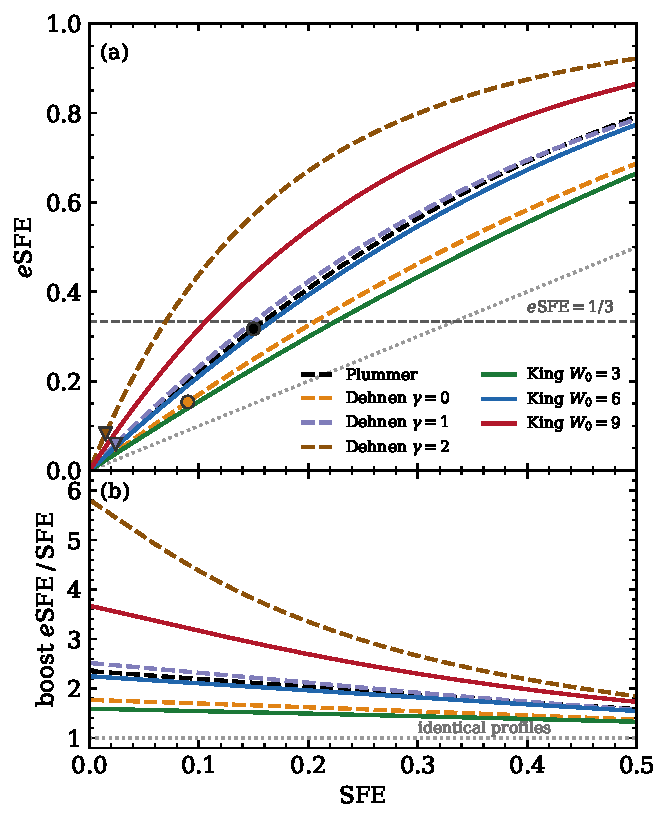
\includegraphics[width=\hsize]{figures/fig8b_esfe_cross_profile.pdf}
\caption{\emph{(a)} Effective against global SFE. Solid, the King models of this
paper; dashed, the published families, with circles at their measured
thresholds and triangles where the published value is a lowest-simulated
upper limit. The horizontal line is $\esfe_{\rm surv}=1/3$; if it were
universal every marker would lie on it. \emph{(b)} The same curves as the
boost factor $\esfe/\sfe$, which resolves the low-SFE corner and tends to
$1/\eta$ as $\sfe\rightarrow0$; dotted line, identical profiles. The
abscissa is the total SFE for King and $\sfe_{10}$ for the published
families throughout. See Sect.~\ref{sec:crossprofile}.}
\label{fig:crossprofile}
\end{figure}

%-------------------------------------------------------------------
\subsection{The King virial threshold curve and its mechanism}
\label{sec:mechanism}

Adopting the classical $\esfe_{\rm surv}=1/3$, the King virial threshold
is the solid ``no truncation'' curve of
Fig.~\ref{fig:truncation} (Sect.~\ref{sec:truncation}, where the
free-fall-time truncation is added as the dashed curve). It is
\emph{non-monotonic}: it decreases from $0.249$ at $W_0=0.5$ to a
minimum of $\sfe_{\rm vir}=0.106$ at $W_0=8.8$, rises to a local
maximum of $0.137$ near $W_0\simeq13.5$, and settles around $0.13$ at
high $W_0$. The simulated grid of Paper~I ($W_0=3,6,9$; predicted
thresholds $0.225$, $0.166$, $0.106$; grey verticals in
Fig.~\ref{fig:truncation}) brackets the descent into the minimum.

Figure~\ref{fig:mechanism} traces the causal chain behind the minimum.
Panel~(c) verifies the exact reduction of Eq.~(\ref{eq:reduction}): the
measured threshold curve coincides with $\eta/(\eta+2)$ to numerical
precision, so the question reduces to the behaviour of $\eta(W_0)$
(panel~b), which reaches a minimum of $\eta=0.238$ at $W_0=8.8$ -- there
the residual gas binds the stars roughly four times less effectively
than identically distributed gas would. The same quantity is what
Fig.~\ref{fig:crossprofile}b displays from the other side: the boost
factor $\esfe/\sfe$ tends to $1/\eta$ as $\sfe\rightarrow0$, so its
intercept reads $\eta$ off directly, giving $1/\eta=1.59$, $2.25$ and
$3.66$ for $W_0=3$, $6$ and $9$. Panel~(a) shows the geometric
origin: the gas--star segregation, measured by
$r_{\rm h,gas}/r_{\rm h,\star}$, peaks (at a value of $3.0$) near
$W_0\simeq8.2$, closely tracking the well-known maximum of the King
structural ratio $\rtid/\rhalf$ at $W_0\simeq8.0$.

The physical picture is as follows. With rising $W_0$ the King model
develops a dense core, and the local-SFE relation places the residual
gas in the increasingly extended, stellar-poor envelope: by the shell
theorem, gas outside the bulk of the stars does not bind them, and
$\eta$ falls. Beyond $W_0\simeq8$, however, the stellar half-mass radius
itself migrates rapidly outward into the developing $r^{-2}$ halo --
this is precisely why $\rtid/\rhalf$ turns over -- so a growing fraction
of \emph{stars} sits in the gas-rich envelope, the segregation
reverses, and $\eta$ rises again, saturating as the model approaches
self-similar isothermal structure. The small offsets between the extrema
(segregation at $W_0=8.2$; $\eta$ and $\sfe_{\rm vir}$ at $8.8$) arise
because $\eta$ weights the segregation by the energy integrand of
Eq.~(\ref{eq:wsg}) rather than by mass alone.

Because $\rtid/\rhalf$ is a property of the King family alone --
independent of the star formation model -- we expect a resilience
optimum near $W_0\simeq8$--$9$ in gas expulsion scenarios in which the
residual gas remains preferentially extended relative to the stars,
whatever mechanism produces that segregation. The argument does not by
itself extend past our other idealizations -- spherical symmetry,
velocity isotropy, and instantaneous removal -- whose relaxation is a
question for the $N$-body campaign.

\begin{figure}[t]
\centering
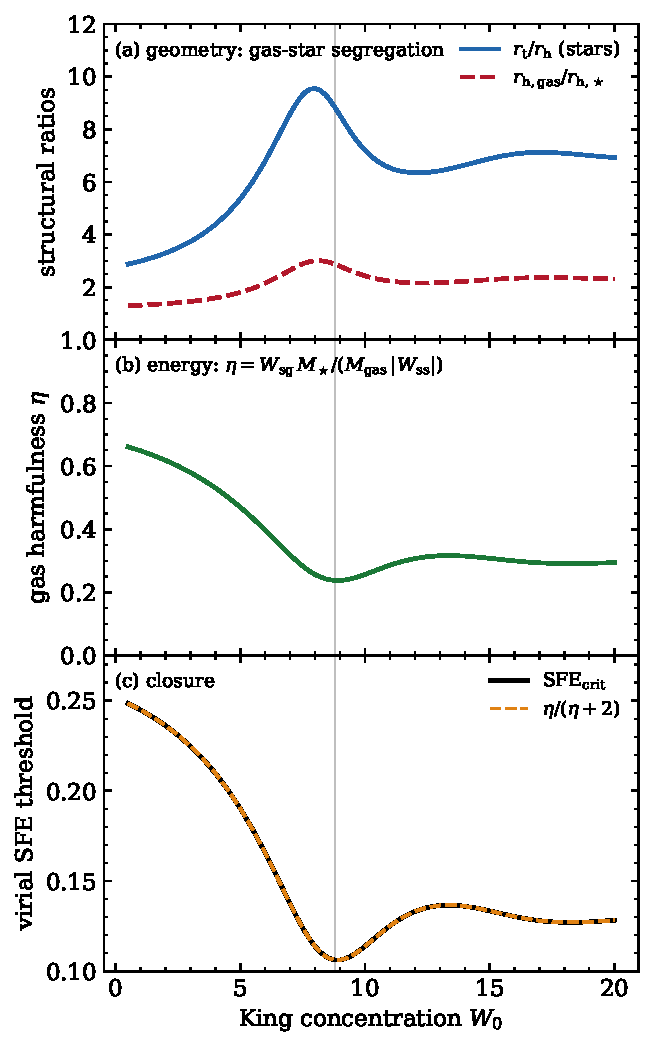
\includegraphics[width=\hsize]{figures/fig6_mechanism.pdf}
\caption{Mechanism of the non-monotonic SFE threshold.
(a)~Structural ratios: $\rtid/\rhalf$ of the stars and the gas--star
segregation $r_{\rm h,gas}/r_{\rm h,\star}$ (scaled $\times5$) at the
threshold configuration. (b)~Gas harmfulness $\eta$
(Eq.~\ref{eq:eta}). (c)~Algebraic consistency check: the computed
$\sfe_{\rm vir}$ coincides with
the exact reduction $\eta/(\eta+2)$. The vertical line marks the minimum
at $W_0=8.8$.}
\label{fig:mechanism}
\end{figure}

\subsection{No universal cluster-wide criterion}
\label{sec:corefraction}

A single cluster-wide $\esfe_{\rm surv}$ is a coarse survival criterion: it
is the dense, gas-poor \emph{centre} of a concentrated model that stays
bound, not the cluster as a whole. Figure~\ref{fig:cumesfe} shows the
cumulative effective SFE $\esfe(<r)$ against the enclosed stellar mass
fraction at each published family's survival threshold. The curves do
not share a common crossing, so no cluster-wide static energy statistic
is universal across profiles.

A natural refinement is to ask whether a fixed \emph{fraction} of the
stellar mass -- the part in a sufficiently bound inner region -- is the
profile-independent invariant. It is not. The stellar mass fraction
interior to the radius where the enclosed SFE falls to $1/3$ is $0.54$
for Plummer but only $0.08$, $0.002$ and $0.07$ for Dehnen
$\gamma=0,1,2$ at their measured thresholds; measured instead against
$\esfe(<r)=1/3$ the fractions are $0.89$, $0.14$, $0.004$ and $0.15$.
Either way the fraction scatters by more than an order of magnitude and
tracks how far each global $\esfe$ sits from $1/3$ rather than revealing
a new constant. The virial statistic, cluster-wide or as a cumulative
inner-core fraction, therefore cannot by itself set the King threshold;
a dynamical calculation is needed, which we provide in
Sect.~\ref{sec:df}.

\begin{figure}[t]
\centering
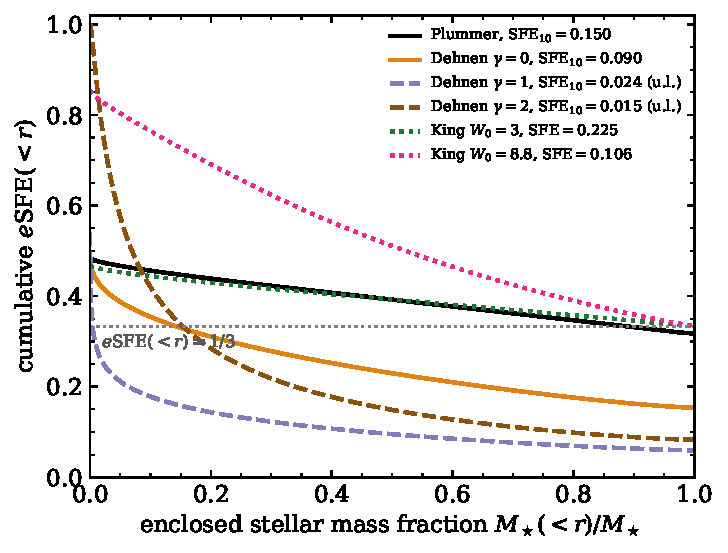
\includegraphics[width=\hsize]{figures/fig8_cumulative_esfe.pdf}
\caption{Cumulative effective SFE, $\esfe(<r)$ -- the ratio of virial
integrals taken inside $r$, not an enclosed star formation efficiency --
as a function of the
enclosed stellar mass fraction, evaluated at each published family's
survival threshold (dashed: censored thresholds). Dotted curves show
King models at their predicted thresholds ($\esfe_{\rm surv}=1/3$). The
curves do not share a common crossing, so no cluster-wide static energy
criterion is universal across profiles.}
\label{fig:cumesfe}
\end{figure}

%-------------------------------------------------------------------
\section{Bound fraction from the distribution function}
\label{sec:df}
%-------------------------------------------------------------------

The virial statistic of Sect.~\ref{sec:esfe} characterizes the cluster
as a whole and, as Sect.~\ref{sec:crossprofile} showed, cannot by itself
account for the survival of centrally concentrated models at low global
$\esfe$. Following \citet{Adams2000} and \citet{BoilyKroupa2003a} we
therefore also compute the bound fraction directly from the stellar
distribution function (DF). This is a second \emph{static} estimator,
not a dynamical calculation: the stellar positions are held fixed while
the gas potential is removed and the escape condition is applied, so
violent relaxation, revirialization and the recapture of marginally
unbound stars are all absent by construction. Closing that gap requires
the live $N$-body campaign of Paper~I.

\subsection{Method}
\label{sec:dfmethod}

The isotropic DF $f(\epsilon)$ is obtained by Eddington inversion
\citep[e.g.][]{BinneyTremaine2008} of the
stellar density in the total (star $+$ gas) relative potential
$\Psi_{\rm tot}$. Rather than differencing a tabulated
$\rho_\star(\Psi)$ twice -- which is ill-conditioned for concentrated
models, since the second-difference stencil is set by the inversion
resolution and refining it amplifies noise -- we evaluate the two
required derivatives $d\rho_\star/d\Psi$ and $d^2\rho_\star/d\Psi^2$ in
closed form via the chain rule through radius. The King density
derivatives $\hat\rho'(W)$ and $\hat\rho''(W)$ are known analytically
(and checked symbolically); $dW/dr$ and $d^2W/dr^2$ are read directly
from the King structure equation; and the potential derivatives follow
from Gauss's law, $\Psi'(r)=-M(r)/r^2$ and
$\Psi''(r)=-4\pi\rho(r)+2M(r)/r^3$. The remaining energy integral in
Eddington's formula is evaluated on a geometric grid after a
$q=\epsilon-\Psi_{\rm t}$ substitution that removes the integrable
square-root singularity analytically. The inversion reproduces the
analytic Plummer DF to a maximum relative error of $6\times10^{-6}$
(Appendix~\ref{app:num}).

At expulsion the DF is frozen, and a star is bound if
$v^2/2<\Psi_{\rm b}(r)$, where $\Psi_{\rm b}$ is generated by the bound
stars only. Removing unbound stars shallows the potential, so the
criterion is iterated to convergence at fixed stellar positions, with
the density of retained stars capped by the initial stellar density.
Every inversion is checked for self-consistency by reconstructing
$\rho_\star$ from the recovered DF; an evaluation is accepted only if
its reconstruction error stays below one per cent over
$0.01<M_\star/M<0.95$, and is otherwise recomputed on a refined energy
grid (a $2000\rightarrow8000\rightarrow32000$-point ladder, applied only
where needed). With this scheme every continuum DF threshold used in the
paper passes the one-per-cent check: the King family at $W_0=0.5$--$20$,
the four published families, and the dense $W_0=2.5$--$20$ scan behind
Figs.~\ref{fig:allthresholds} and~\ref{fig:validation}, with a
worst-case reconstruction error of $1.0$ per cent.

This frozen-DF estimate neglects violent relaxation, revirialization,
and the recapture of outflowing stars. For identical star and gas
profiles it reproduces the known sharp analytic transition, retaining a
bound remnant only for $\sfe\gtrsim0.4$--$0.5$
\citep{BoilyKroupa2003a}; it is thus \emph{conservative} relative to
$N$-body results in that regime.

\subsection{King family: DF versus virial threshold}
\label{sec:dfking}

Figure~\ref{fig:fbound} shows the resulting bound fraction
$F_{\rm b}(\sfe)$ for the King family, and Fig.~\ref{fig:allthresholds}
compares the DF-based threshold (defined by $F_{\rm b}<0.02$) with the
virial one. The level $F_{\rm b}=0.02$ is an operational definition of
the frozen-DF transition, not a claim about a universal survival
fraction. Where $F_{\rm b}(\sfe)$ rises steeply -- $W_0\lesssim10$,
covering the whole non-monotonic descent and the $W_0=3,6,9$ grid of
Paper~I -- moving the cut between $0.01$ and $0.05$ shifts the threshold
by at most $0.007$ in $\sfe$; for the most concentrated models the rise
is gradual and the shift reaches $0.023$, so those values are indicative
only. The non-monotonicity survives at every cut in that range, with
only the location of the broad minimum drifting between $W_0\simeq10$
and $\simeq16$. The two criteria measure
different physics and diverge
strongly with concentration. For $W_0\lesssim5$ the DF threshold lies
\emph{above} the virial one -- frozen-DF conservatism dominates -- while
for concentrated models it falls far below it, to
$\sfe_{\rm DF}\simeq0.048$ at $W_0=9$ and a broad minimum of
$\simeq0.018$ near $W_0\simeq13$, against virial values of $0.106$ and
$0.129$. The two criteria therefore have their minima at different
concentrations -- $W_0=8.8$ for $\sfe_{\rm vir}$
(Sect.~\ref{sec:mechanism}) and $W_0\simeq13$ for $\sfe_{\rm DF}$ -- and
the two should not be conflated: the first is where gas--star segregation
is most effective, the second where the surviving central seed is
densest. The dense, gas-poor centre retains a self-bound seed even when
the cluster as a whole is formally super-virial. This is precisely the
mechanism required by Sect.~\ref{sec:crossprofile}: applied to the
published thresholds, the frozen-DF estimate leaves the cuspy Dehnen
$\gamma=2$ model marginally bound ($F_{\rm b}\simeq0.03$) at its
measured threshold, while dissolving the shallower Plummer and Dehnen
$\gamma=0,1$ cases -- reproducing the \emph{ordering} of the published
thresholds across profiles, though not their exact values. The
DF-based thresholds of the published families are
$\sfe_{\rm DF}=0.193$ (Plummer), $0.158$ ($\gamma=0$),
$0.079$ ($\gamma=1$) and $0.009$ ($\gamma=2$), i.e.\ $1.3$ and $1.8$
times the measured Plummer and Dehnen $\gamma=0$ $N$-body thresholds
(Sect.~\ref{sec:nbodyvalid}).

\subsection{Monte Carlo verification and finite-$N$ effects}
\label{sec:mc}

We checked the frozen-DF predictions against Monte Carlo realizations of
the actual initial conditions: for each $(W_0,\sfe)$ configuration,
$N=10^5$ equal-mass particles were sampled from the quasi-spherical DF in
the total potential with \textsc{Agama} \citep{Vasiliev2019} -- the same
machinery that generates the $N$-body initial conditions of Paper~I --
and the iterated escape criterion applied particle-wise. Every quoted
particle result uses $150$ realizations at this $N$; smaller $N$ appears
only in the scaling experiment below.

On the developed branch ($F_{\rm b}\gtrsim0.1$) the continuum agrees with
the realizations to better than one per cent absolute at $W_0=3,9,12$
(Fig.~\ref{fig:validation}), validating the inversion, the sampling and
the criterion together. The $2$--$4$ per cent excess at $W_0=6$ is not an
inversion error: the continuum turns on $\Delta\sfe\simeq0.012$ earlier
in SFE than the discrete systems, and where the curve is near-vertical --
as it is most sharply at $W_0=6$ -- that horizontal offset reads as a
vertical gap. The same offset is negligible at $W_0=9,12$, and so is the
gap.

The threshold is taken as the SFE at which the survival fraction
$p=P(F_{\rm b}>0.02)$ crosses one half. Because the transition is narrow
at $N=10^5$ -- at $W_0=3$ it completes within $\Delta\sfe=0.005$ -- the
SFE grid was refined around each crossing until several points fell
inside the transition, so that the interpolation is not the limiting
uncertainty. The error is then obtained by bootstrapping over
realizations: the $150$ outcomes at each SFE are resampled with
replacement, $p$ is re-formed and the crossing re-interpolated, and we
quote the $16$th--$84$th percentile spread. This propagates the binomial
sampling noise of every grid point through the interpolation, and it
does not assume a centre for the strongly bimodal cells, where a mean
$F_{\rm b}$ has none. The result, marked in
Fig.~\ref{fig:allthresholds}, is
\begin{equation}
  \sfe_{\rm DF} = 0.3028,\; 0.1897,\; 0.0477,\; 0.0193
  \quad (W_0=3,6,9,12),
  \label{eq:mcthresh}
\end{equation}
with bootstrap uncertainties of $1.1$, $1.3$, $0.6$ and
$0.6\times10^{-4}$ respectively. An independent estimate,
$\sigma_p/|dp/d\sfe|$ with $\sigma_p=\sqrt{p(1-p)/150}$, agrees with the
bootstrap to about $30$ per cent. These are the values used wherever
frozen-DF Monte Carlo thresholds are quoted
(Sects.~\ref{sec:disc_predictions} and~\ref{sec:conclusions}).

That precision belongs to the estimator, not to the prediction. The
frozen-DF thresholds sit $1.3$--$1.8$ times above the measured $N$-body
values for the published families (Sect.~\ref{sec:nbodyvalid}), a
model-level discrepancy some three orders of magnitude larger than these
error bars.

The transition is intrinsically stochastic at finite $N$, and the
stochasticity is itself $N$-dependent. Holding the configuration fixed
just below the large-$N$ threshold and varying only the particle number,
the survival probability falls monotonically over more than two decades:

\begin{center}
\begin{tabular}{lcccccc}
\hline\hline
$N$ & $10^3$ & $3\times10^3$ & $10^4$ & $3\times10^4$ & $10^5$ & $3\times10^5$\\
\hline
$W_0=3$  & 0.58 & 0.49 & 0.35 & 0.11 & 0.00 & 0.00\\
$W_0=9$  & 0.63 & 0.49 & 0.23 & 0.03 & 0.00 & 0.00\\
\hline
\end{tabular}
\end{center}

\noindent
($150$ realizations per entry, binomial errors $\le0.041$; $W_0=3$ at
$\sfe=0.30$ and $W_0=9$ at $\sfe=0.045$). Shot noise in the potential of
the bound subset occasionally carries a sub-threshold realization into
the basin of the surviving branch, and the chance of that happening
vanishes as the sampling noise does. A diffuse and a concentrated model
give the same decline, so this is a property of the family rather than
of one configuration. The same stochasticity, augmented by violent
relaxation, will govern the marginal cells of the $N$-body grid
($N\simeq1.7\times10^4$ in Paper~I), for which the survival
\emph{probability} across realizations, rather than a sharp threshold,
is the observable to measure.

The threshold itself, however, does not move with $N$. Repeating the
measurement at $N=3\times10^5$ shifts it by $-8\times10^{-5}$ at $W_0=3$
and $+7\times10^{-5}$ at $W_0=6$ -- smaller than the bootstrap
uncertainties quoted above, and of opposite sign, as scatter about a
converged value rather than a drift. What tripling $N$ does change is the
\emph{width} of the transition, which falls from $\Delta\sfe=0.0030$ to
$0.0017$ at $W_0=3$ and from $0.0020$ to $0.0011$ at $W_0=6$ (the SFE
interval over which $p$ runs from $0.1$ to $0.9$). Both ratios, $0.565$
and $0.557$, match the $N^{-1/2}$ expected of pure sampling noise
($3^{-1/2}=0.577$) to within four per cent. Finite $N$ therefore smears a
fixed threshold symmetrically rather than displacing it, which is why the
median crossing is the appropriate estimator: a definition keyed to the
onset of survival would track the tail of that smearing and drift with
$N$. This was verified at $W_0=3$ and $6$, so the convergence of
Eq.~(\ref{eq:mcthresh}) is established at those two concentrations and
assumed at the other two, where the transition has the same character. It
is
also the same effect as the table above seen from the other side -- at a
fixed SFE below the centre, a narrowing distribution leaves less
probability above the survival cut, so $p$ falls with $N$.

\begin{figure}[t]
\centering
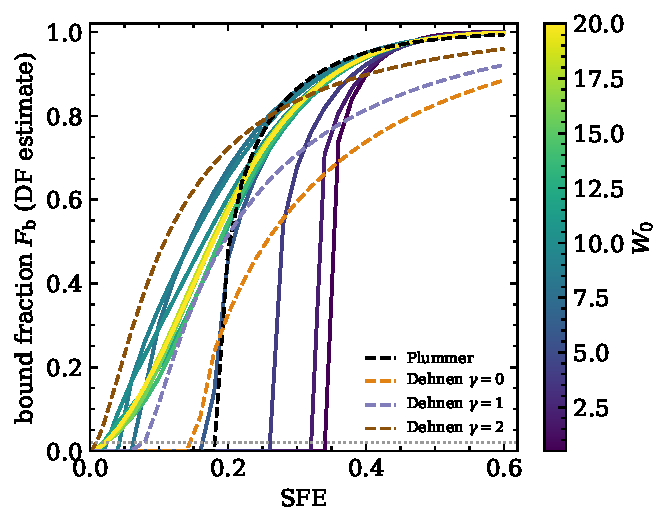
\includegraphics[width=\hsize]{figures/fig10_fbound_curves.pdf}
\caption{Bound fraction after instantaneous gas expulsion, estimated
from the frozen distribution function with the iterated escape
criterion, as a function of the global SFE for King models with
$W_0=0.5$--$20$. The global SFE here is measured within the tidal radius
(the infinite-extent published families elsewhere in this paper use
$\sfe_{10}$). The dotted line marks the $F_{\rm b}=0.02$ level used to
define the DF-based threshold.}
\label{fig:fbound}
\end{figure}

\begin{figure}[t]
\centering
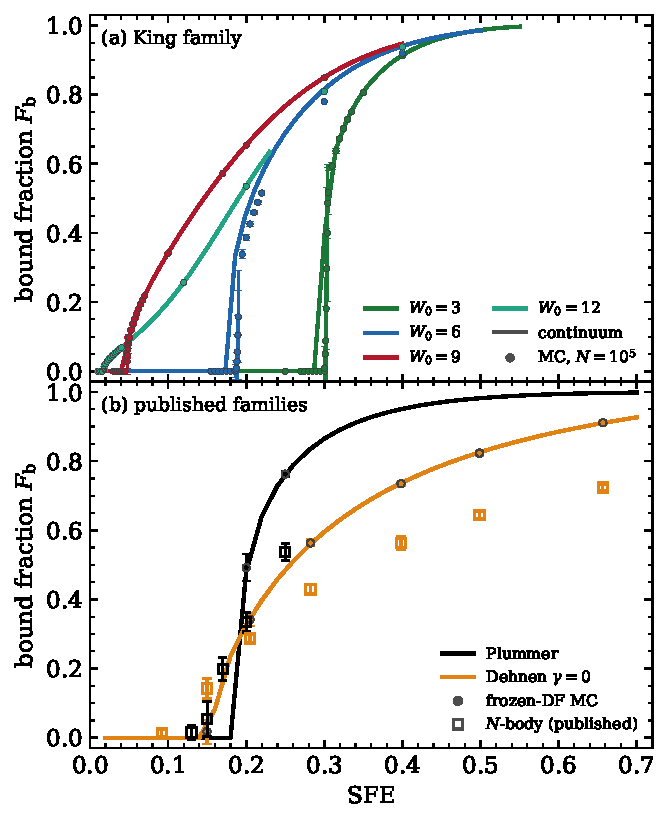
\includegraphics[width=\hsize]{figures/fig12_validation.pdf}
\caption{Verification of the frozen-DF bound fraction. Curves, the continuum
calculation; points, mean $\pm$ standard deviation over $150$
realizations of $N=10^5$ particles; the abscissa is the total SFE in (a)
and $\sfe_{10}$ in (b).
\emph{(a)} King family (Sect.~\ref{sec:mc}).
\emph{(b)} The two published families with $N$-body measurements, whose
results are the open squares (Sect.~\ref{sec:nbodyvalid}).}
\label{fig:validation}
\end{figure}

\begin{figure}[b]
\centering
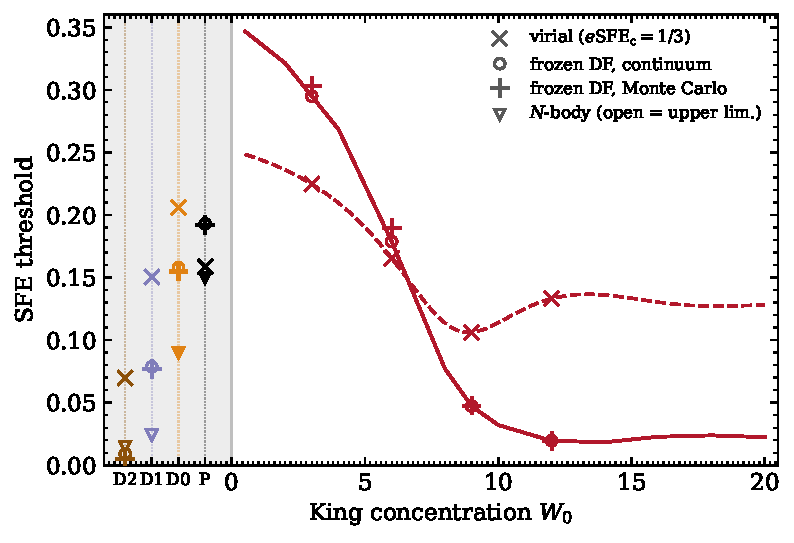
\includegraphics[width=\hsize]{figures/fig11b_thresholds_with_mc.pdf}
\caption{SFE thresholds from every criterion considered. King family in red
(dashed, virial; solid, frozen-DF continuum); the published families
occupy the strip left of $W_0=0$ at ordinal positions (P, D0, D1, D2),
where the abscissa carries no meaning. Symbols: $\times$ virial,
$\circ$ frozen-DF continuum, $+$ frozen-DF Monte Carlo,
$\triangledown$ published $N$-body (open where that value is an upper
limit). The ordinate is criterion-specific; the shaded strip is where the
SFE convention changes from the King total value to $\sfe_{10}$. None of the
plotted values is the critical SFE in the dynamical sense
(Sect.~\ref{sec:disc_criteria}).}
\label{fig:allthresholds}
\end{figure}

\subsection{Confrontation with $N$-body results}
\label{sec:nbodyvalid}

For the Plummer and Dehnen $\gamma=0$ families the bound fraction has
been measured directly in $N$-body simulations, so the frozen-DF estimate
can be tested rather than merely bracketed (Fig.~\ref{fig:validation}).
Two things follow.

First, the Monte Carlo and the continuum agree with each other to
$\lesssim0.01$ in $F_{\rm b}$ at every simulated SFE, and their published
thresholds to about one per cent ($0.193$ vs.\ $0.192$ for Plummer;
$0.158$ vs.\ $0.155$ for Dehnen $\gamma=0$). That rules out sampling
noise and the marginal-branch sensitivity of Sect.~\ref{sec:mc} as
explanations for the offset from the $N$-body points, leaving the physics
the frozen distribution function omits as the natural candidate -- though
the comparison alone cannot exclude residual differences in the initial
conditions or in how bound mass is measured.

Second, that separation is systematic and changes sign at the
threshold. Below it the frozen DF dissolves clusters that survive in the
simulations (at $\sfe_{10}=0.17$ the Plummer runs retain
$F_{\rm b}\simeq0.2$ where both frozen-DF estimates give zero); above it
the frozen DF overpredicts the surviving mass, by $+0.15$ and $+0.22$ at
$\sfe_{10}=0.20$ and $0.25$ for Plummer, and by a nearly constant
$+0.13$--$+0.19$ across $\sfe_{10}=0.28$--$0.66$ for Dehnen $\gamma=0$
(from a dedicated Monte Carlo comparison at the published $N$-body SFE
values; Fig.~\ref{fig:validation}). Both signs share one origin. The frozen DF holds the stars at fixed
positions and lets the potential shallow as members are removed, so it
misses the revirialization that lets a marginal cluster re-form a bound
core -- hence the missing survivors below threshold -- while also
ignoring the further mass loss revirialization imposes on a cluster that
does survive -- hence the excess above it. The corresponding thresholds
are $1.3$ and $1.8$ times the measured $N$-body values for Plummer and
Dehnen $\gamma=0$ respectively.

Underlying both signs is a structural property of the frozen estimate:
it is bistable, and the live system is not. The escape condition is
solved self-consistently -- which stars are bound given the potential of
the stars that are bound -- and that iteration is self-amplifying, since
unbinding a star shallows the potential and unbinds more. It therefore
is observed to settle on one of only two outcomes, complete dissolution
or a self-gravitating remnant, with no intermediate state persisting: a
configuration retaining a small fraction of its stars keeps unbinding.
Below a critical SFE the second outcome disappears, and $F_{\rm b}$
therefore does not rise continuously from zero. We report this
empirically, as a property of the iteration we solve; the fixed-point
analysis that would establish the bifurcation structure formally has not
been carried out here.

The particle realizations show this directly. Through the entire
transition at $W_0=3$ every realization either dissolves completely or
retains $F_{\rm b}\simeq0.45$--$0.52$, with nothing in between: at
$\sfe=0.3025$, $58$ of $150$ realizations survive with
$F_{\rm b}=0.469\pm0.062$ and the other $92$ give exactly zero. What
sweeps across the transition is the \emph{proportion} of survivors, not
the bound fraction of a survivor, so the ensemble mean rises smoothly
only as a mixture of zeros and halves and describes no individual
cluster. The iteration count carries the same signature: convergence
takes $16$ iterations well below threshold and $11$ well above it, but
over $130$ at the transition, the critical slowing down expected where
two fixed points merge.

Live $N$-body clusters do not behave this way -- the published Plummer
sequence passes smoothly through $F_{\rm b}=0.015$, $0.054$, $0.199$,
$0.334$ and $0.538$ as $\sfe_{10}$ runs from $0.13$ to $0.25$. Violent
relaxation and revirialization let a remnant settle at an intermediate
bound fraction that is dynamically reachable but is not a fixed point of
the frozen map. The discontinuity is therefore a property of the
approximation rather than of the physics, and it is the reason the
frozen-DF threshold sits above the measured one: at $\sfe_{10}=0.17$ the
frozen estimate must return zero, because the only alternative available
to it is a fully-formed remnant.

The correction is thus not a single number: it depends on the profile
and on which side of the threshold one sits, exactly as the
non-universality of Sect.~\ref{sec:crossprofile} would suggest. We
therefore quote the frozen-DF results as what they are -- an upper bound
on the surviving mass of a surviving cluster, and an empirical upper
estimate of the critical SFE, calibrated on the published comparison
rather than proved -- and expect the $N$-body thresholds of Paper~I to
fall below the Monte Carlo values of Sect.~\ref{sec:mc}, by a factor of
order $1.3$--$1.8$ if the published families are any guide.

%-------------------------------------------------------------------
\section{A free-fall-time truncation criterion}
\label{sec:truncation}
%-------------------------------------------------------------------

The criterion of this section is a sensitivity experiment: we impose a
hard boundary at $\tff=\tsf$ to bound how much the results can depend on
gas that had no time to form stars. It is not a claim that star
formation switches off discontinuously at that density, and the
untruncated model of Sect.~\ref{sec:gas} remains the baseline
throughout.

The local-SFE relation of Sect.~\ref{sec:gas} presumes that the gas at
every radius has had time to reach the local star formation efficiency
per free-fall time. Where the local free-fall time exceeds the star
formation duration, $\tff(r)>\tsf$, this presumption fails. The
condition $\tff=\tsf$ translates into a scale-free contrast against the
central gas plateau of Eq.~(\ref{eq:gas}),
$\rho_{\rm plat}\equiv k^{-2}=3\pi/(8G\effE^2\tsf^2)$, namely
\begin{equation}
  \frac{\rho_{\rm SF}}{\rho_{\rm plat}} = \frac{\effE^2}{4},
  \label{eq:trunc}
\end{equation}
independent of $\tsf$, of the clump mass, and of all radial scales: the
truncation is scale-free and controlled by $\effE$ alone. At the
observationally favoured $\effE=0.01$ the contrast is only
$2.5\times10^{-5}$, so the star-forming region extends to very low gas
density and the truncation is a small correction; at the legacy
$\effE=0.05$ it is a factor $25$ stronger.

This is the only place $\effE$ can matter. It enters the gas profile
solely through $k=\sqrt{8/(3\pi)}\,\effE\,\tsf$ (Eq.~\ref{eq:k}), so a
change of $\effE$ is \emph{exactly} equivalent to a relabelling of
$\tsf$, and every untruncated result of this paper -- the
$\esfe$--$\sfe$ relations, the threshold curves, the location of the
minimum -- is rigorously independent of it. Figure~\ref{fig:truncation}b
shows the truncated curve for $\effE=0.01$, $0.05$ and $0.10$: as
$\effE\rightarrow0$ the truncation becomes irrelevant and the curve
converges to the untruncated result (minimum $\sfe_{\rm vir}=0.108$ at
$W_0=9$ for $\effE=0.01$, against $0.106$ at $W_0=8.8$ untruncated),
while larger $\effE$ removes more envelope gas, raising the thresholds
and shifting the minimum to higher concentration ($0.16$ at
$W_0\simeq10$ for $\effE=0.05$; $0.25$ at $W_0\simeq13$ for $0.10$). The
non-monotonicity survives for every value considered. For the published
families the same sweep sets the minimum reachable $\sfe_{10}$ under the
removal flavour: for $(\effE=0.01,\,0.05,\,0.10)$ it is
$(0.026,\,0.123,\,0.228)$ for Plummer, $(0.029,\,0.136,\,0.253)$ for
Dehnen $\gamma=0$, $(0.033,\,0.153,\,0.280)$ for $\gamma=1$ and
$(0.041,\,0.185,\,0.329)$ for $\gamma=2$.

Two implementations must be distinguished. In the \emph{removal} flavour,
gas at $r>\rsf$ (where $\rho_{\rm g}=\rho_{\rm SF}$) is excluded from the
potential entirely. Applied to the Dehnen models of S21 -- whose total
gas mass otherwise diverges as $r^{1/3}$, Eq.~(\ref{eq:trunc}) providing
a physical regularization -- the reachable $\sfe_{10}$ then has a minimum
of $0.029$, $0.033$ and $0.041$ for $\gamma=0,1,2$. The Dehnen
$\gamma=0$ threshold ($\sfe_{10}=0.090$) is comfortably above this floor
and is therefore realizable under the removal flavour; only the two
$\gamma\ge1$ cases -- both censored upper limits -- lie below it. (At
the legacy $\effE=0.05$ the floors rise to $0.123$--$0.185$, which
forbids the three Dehnen configurations but still leaves the Plummer
threshold, $\sfe_{10}=0.150$, above its floor of $0.123$; only at
$\effE=0.10$ is every published configuration excluded.) In the \emph{aperture} flavour the
dynamics retain the full gas distribution and $\rsf$ only bounds the
region within which the clump and its SFE are measured; a third variant
additionally reassigns the stellar mass beyond $\rsf$ to gas (those
stars are not yet meant to have formed), which lowers the global SFE to
the stellar mass fraction within $\rsf$ times $\sfe_{10}$. Neither
compresses the factor-of-ten spread of the published thresholds at
$\effE=0.01$, where $\rsf$ is large and $\sfe(<\rsf)\rightarrow\sfe_{10}$.

For the King family the gas is finite in any case, and because $\rsf$
falls close to $\rtid$ the three variants very nearly agree: essentially
no stellar mass lies beyond $\rsf$ at threshold
($M_\star(<\rsf)/M_\star\ge0.999$ for $W_0=3$--$12$), so the third
variant lowers the global SFE by $\le0.0002$, and removal differs from
the aperture reading by no more than the $0.002$ quoted below. They are
not identical, but the distinctions that matter for the published
families are immaterial here. Figure~\ref{fig:truncation} compares the
threshold curve with and without the removal-flavour truncation. At $\effE=0.01$ the two curves are
nearly indistinguishable: truncation raises the threshold by at most
$0.002$ and does not move the minimum, which stays at $W_0\simeq9$. The
star-forming radius reaches close to the tidal radius,
$\rsf/\rtid=0.81$--$0.98$ at threshold, so the mild internal tension of
the assumed King profile extending past $\rsf$
(Sect.~\ref{sec:disc_selfcons}) is confined to the outermost few per
cent of the cluster. The non-monotonicity -- the central result of this
paper -- is untouched.

\begin{figure}[b]
\centering
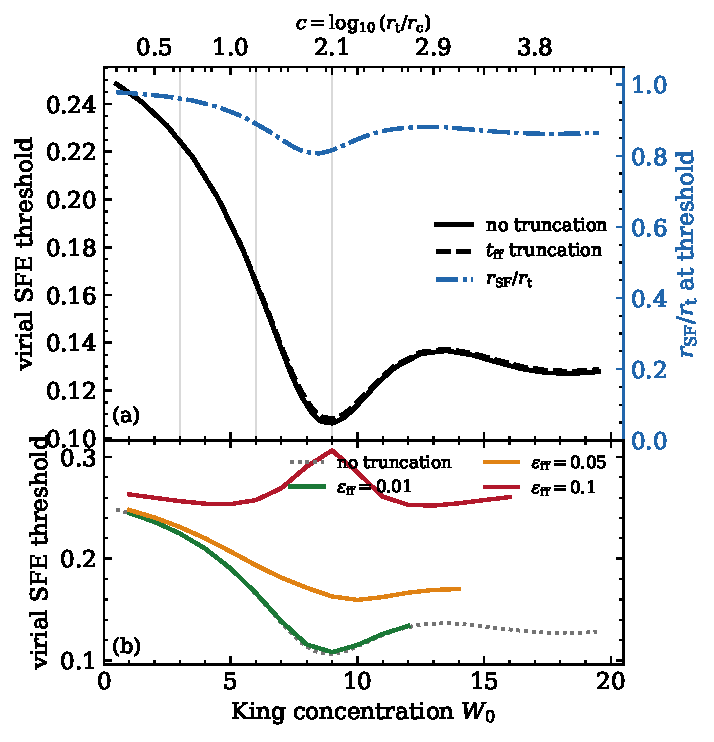
\includegraphics[width=\hsize]{figures/fig9_truncation.pdf}
\caption{\emph{(a)} Virial SFE threshold with and without the free-fall-time
truncation (removal flavour; black solid and dashed) at the fiducial
$\effE=0.01$, and the star-forming radius $\rsf/\rtid$ at the threshold
configuration (blue dash-dot, right axis). Grey verticals mark the
Paper~I grid ($W_0=3,6,9$); the top axis carries
$c=\log_{10}(r_{\rm t}/r_{\rm c})$. \emph{(b)} The truncated curve for
$\effE=0.01$, $0.05$ and $0.10$ against the untruncated result (dotted),
which is exactly independent of $\effE$. See Sect.~\ref{sec:truncation}.}
\label{fig:truncation}
\end{figure}

%-------------------------------------------------------------------
\section{Discussion}
\label{sec:discussion}
%-------------------------------------------------------------------

\subsection{Two static criteria and the true threshold}
\label{sec:disc_criteria}

Section~\ref{sec:corefraction} showed that no static energy statistic --
cluster-wide or as an inner-core fraction -- is universal across density
profiles, because survival of a concentrated system is decided by the
dense, gas-poor centre that retains a self-bound seed even when the
cluster as a whole is formally super-virial. The two criteria we can
compute cheaply, the virial ratio and the frozen DF, therefore provide
two complementary reference thresholds whose separation
(Fig.~\ref{fig:allthresholds}) measures the physics that neither
captures: violent relaxation, revirialization, and the recapture of
outflowing stars. Neither is a proven bound on the true threshold. What
the published families do establish is one-sided: wherever the $N$-body
threshold is measured rather than censored it lies below the frozen-DF
value (Plummer $0.150$ versus $0.193$; Dehnen $\gamma=0$, $0.090$ versus
$0.158$), as does the $\gamma=1$ upper limit; only the $\gamma=2$ limit
is uninformative. We therefore expect the King $N$-body thresholds to
fall below their frozen-DF values as well.
Figure~\ref{fig:allthresholds} collects every
criterion -- virial, frozen-DF continuum, frozen-DF Monte Carlo, and the
published $N$-body results -- for the King family and the published
families on a common axis. The two criteria cross near
$W_0\simeq5$--$6$. For diffuse clusters the frozen-DF
estimate is conservative (it disrupts the Plummer model at its measured
$N$-body threshold) and the virial criterion is the closer guide; for
concentrated clusters the situation reverses, with the virial criterion
overestimating the threshold by about a factor of two at $W_0=9$
($0.106$ versus $0.047$). Paper~I will locate the true $N$-body
threshold relative to this pair; combining its grid with the S17/S21
points should then allow $\esfe_{\rm surv}$ to be calibrated as an explicit
function of a concentration measure, restoring the usefulness of the
energy criterion in a profile-dependent form.

Finally, the Monte Carlo experiments of Sect.~\ref{sec:mc} show that
close to threshold the very notion of a sharp critical SFE dissolves:
survival becomes a probability over realizations, with shot noise able
to rescue sub-threshold clusters at low $N$. This stochasticity is not a
numerical artefact but a property of the discrete problem. We caution
that the trend was measured at two concentrations only, and that the
survival probability is a property of the frozen escape criterion rather
than of a live cluster. Whether real low-$N$ clusters, which span
$N\sim10^2$--$10^6$, show a correspondingly shifted survival probability
is a question for live $N$-body experiments rather than a result of this
work.

\subsection{Robustness to the expulsion timescale, $\effE$, and
isotropy}
\label{sec:disc_robust}

Three model assumptions deserve scrutiny. First, instantaneous
expulsion: coupled simulations find feedback-driven expulsion to proceed
on roughly a clump free-fall time \citep{Li2019}, dynamically close to
the impulsive limit \citep{BaumgardtKroupa2007}, and
\citet{Fujii2021c} conclude, by comparing star-by-star cluster formation
against the instantaneous star formation and gas expulsion of
\citet{FujiiPZ2016}, that the simplified treatment is sufficient for the
dynamical evolution of clusters after gas expulsion. Slower expulsion
raises all bound fractions \citep{BaumgardtKroupa2007}, so our
thresholds are conservative in that respect; whether its $W_0$-dependent
magnitude preserves the non-monotonic \emph{shape} is not established
here, since a correction of one sign can still vary with concentration
enough to move or erase an extremum. The predictions of this paper
therefore apply specifically to the instantaneous-expulsion limit. Second, $\effE$: by the exact
degeneracy of Sect.~\ref{sec:truncation}, every untruncated result is
rigorously independent of it, and the truncated threshold curves remain
non-monotonic across the full observationally reported range
$\effE=0.01$--$0.10$ (Fig.~\ref{fig:truncation}b). Third, isotropy: the
initial conditions are isotropic by construction, matching the $N$-body
models of Paper~I; primordial velocity anisotropy would alter the
frozen-DF bound fractions -- \citet{Adams2000} showed radial anisotropy
raises them -- and is a natural extension of the framework that we
defer.

\subsection{Simulation support for the centrally peaked SFE}
\label{sec:disc_sim}

Beyond the analytic argument of \citet{Parmentier2013}, our
MHD$+$$N$-body simulations of this formation channel show, in the
specific setups modelled there, that centrally concentrated clouds
assemble centrally concentrated clusters -- in fact \emph{more} compact ones than the
analytic construction predicts, with fitted Plummer and EFF scale radii
systematically below the input value and a shape well described by a
Plummer profile \citep{Assilkhan2026}. This outcome arises through
global collapse of the gas toward the centre rather than the purely
local conversion assumed by \citet{Parmentier2013}, so the framework of
Sect.~\ref{sec:gas} is supported at the level of the emergent structure
even where its formation mechanism is idealized. The stellar
substructure inherited from the cloud is erased within $\sim$$2.5$
free-fall times by dynamical relaxation \citep{Akhmetali2026},
consistent with treating the cluster as a smooth centrally concentrated
system by the time of gas expulsion. The concentration of the emergent
cluster is, however, sensitive to early feedback physics: including
protostellar jets in otherwise identical initial conditions yields
systematically \emph{less} concentrated outcomes -- more extended, more
substructured, less tightly bound, and more supervirial stellar systems,
with the star formation efficiency suppressed from $19$--$33$ to
$12$--$16$ per cent \citep{AssilkhanJets2026}. Different feedback
channels thus map one and the same clump onto a \emph{range} of emergent
concentrations -- precisely the axis the King $W_0$ family parametrizes,
and the reason cluster survivability must be known across the whole
family rather than at a single fiducial profile.

\subsection{Observational touchpoints}
\label{sec:disc_obs}

Three observational touchpoints already exist. First, the constant-$\effE$
assumption inherited from \citet{Parmentier2013} is directly supported
within nearby clouds: \citet{Pokhrel2021} find
$\Sigma_{\rm SFR}=\effE\,\Sigma_{\rm gas}/\tff$ with $\effE$ nearly
independent of gas density, a median $\effE\simeq0.026$, and a
cloud-to-cloud scatter of only $0.18$~dex, consistent with the earlier
surface-density relation of \citet{Gutermuth2011}; on both sub-galactic and
galaxy-wide scales the value converges to $\effE\simeq0.01$
\citep{KrumholzMcKeeBlandHawthorn2019,Utomo2018}, which we adopt as
fiducial. At the highest column densities the picture is debated, the
CAFFEINE survey finding the SFE to saturate above a critical density
\citep{Mattern2024}; but the exact $\effE$--$\tsf$ degeneracy of
the $\effE$--$\tsf$ degeneracy renders every untruncated result of this
paper immune to the controversy, and only the free-fall-time truncation of
Sect.~\ref{sec:truncation} is exposed to it. Second, the truncation
itself offers a physical reading of the
empirical dense-gas threshold for star formation
\citep{Lada2010,Lada2012}: in our framework the apparent threshold is
not a universal density but a free-fall-time condition,
$\rho_{\rm SF}=3\pi/(32\,G\,\tsf^2)$, predicting that the threshold
should scale with the star formation duration of the clump. Third, the
model predicts the density profile of the \emph{primordial clump}
itself: because the \citet{Parmentier2013} construction holds the total
density fixed while gas is converted into stars -- an assumption built
into Eq.~(\ref{eq:gas}) -- the sum $\rho_\star+\rho_{\rm g}$ is the
initial clump profile, directly comparable to dust-continuum
observations of clumps at early evolutionary stages. Fitting
$\rho\propto r^{-p}$ between the radii enclosing $10$ and $90$ per cent
of the mass yields $p_{\rm tot}\simeq2.2$--$2.5$ across the entire King
family, insensitive to both $W_0$ and the global SFE. This matches the
clump-scale profiles of the youngest observed sources
\citep[$p\simeq2.2$ at the earliest phases;][]{Gieser2023}, classical
single-power-law fits giving a shallower $\langle p\rangle=1.6$--$1.7$
with a documented outward steepening
\citep{Mueller2002,Beuther2002,Pirogov2009}. The near-universality of
the slope is itself a prediction: the envelope slope cannot discriminate
the concentration of the embedded cluster, which is instead encoded in
the density contrast between the central plateau and the clump mean. A
forward-modelled comparison with the ATLASGAL and Hi-GAL clump
populations \citep{Urquhart2018,Elia2021} is deferred to future work.

\subsection{Towards a self-consistent stellar profile}
\label{sec:disc_selfcons}

An internal tension of the model remains. The stellar profile is
\emph{assumed} to be a King model extending to $\rtid$, while the
free-fall-time criterion of Sect.~\ref{sec:truncation} implies that star
formation is confined within $\rsf<\rtid$ (Fig.~\ref{fig:truncation}). A
self-consistent treatment would instead start from the primordial clump
profile, apply the local-SFE relation together with the free-fall-time
criterion, and \emph{derive} the stellar profile -- generally close to,
but not exactly, a truncated King model -- iterating the pair to a fixed
point. We regard this as the principal structural refinement for future
work. A second, more practical lesson of the same kind emerged in
Sect.~\ref{sec:crossprofile}: quoted SFE values depend materially on the
measurement aperture (the S17 threshold is reproduced only under the
$10\,a$ aperture, and the S21 thresholds required an explicit
$\sfe_{\rm J}\rightarrow\sfe_{10}$ conversion), so comparisons of star
formation efficiencies across studies -- observational or numerical --
must state the aperture to be meaningful.

\subsection{Predictions for the $N$-body campaign}
\label{sec:disc_predictions}

The framework makes the following concrete, falsifiable predictions for
the simulation grid of Paper~I ($W_0=3,6,9$;
$N\simeq1.7\times10^4$).
(1)~The virial criterion with $\esfe_{\rm surv}=1/3$ places the virial
threshold at $0.225$, $0.166$, and $0.106$ for $W_0=3,6,9$ (minimum
$0.106$ at $W_0=8.8$); at the fiducial $\effE=0.01$ the free-fall-time
truncation leaves these values unchanged to within $0.002$.
(2)~The frozen-DF Monte Carlo thresholds are $0.3028$, $0.1897$ and
$0.0477$ (plus $0.0193$ at $W_0=12$), each determined to
$\sim\!10^{-4}$;
we expect the measured $N$-body thresholds to lie below the frozen-DF
estimates, as they do for Plummer and Dehnen $\gamma=0$; where they fall
relative to the virial estimate is a prediction to be tested, not a
bracket established here. In particular the
\emph{ordering} of survivability with $W_0$ -- the non-monotonicity --
is the sharpest qualitative test.
(3)~On the developed branch the bound-fraction curves of
Fig.~\ref{fig:validation} are quantitative initial-condition-level
predictions, verified against $N=10^5$ realizations to better than one
per cent for $W_0=3,9,12$ and a few per cent for $W_0=6$; systematic
deviations of the $N$-body results from these curves isolate the
contribution of violent relaxation.
(4)~In the marginal cells, survival should be reported as a probability
over random realizations rather than a binary outcome; at
$N\simeq1.7\times10^4$ the scaling above puts the expected survival
probability near $0.2$--$0.3$ at $W_0=3$, $\sfe=0.30$.
(5)~As a consistency check of the initial-condition pipeline, in the
half-mass-radius units the campaign actually uses ($G=M_\star=r_{\rm h}=1$,
with $\lambda\equiv r_{\rm h}/R_{\rm J}$ held fixed across $W_0$) the
star formation duration required for a given SFE is nearly universal,
$\tsf(\sfe{=}0.17)\simeq23$--$63$ across the whole family
(Fig.~\ref{fig:sfetsf}; factor $\simeq2.7$), the absolute scale set by
the low $\effE$ rather than by the geometry.

%-------------------------------------------------------------------
\section{Conclusions}
\label{sec:conclusions}
%-------------------------------------------------------------------

We have built a King-family initial-condition set for embedded clusters
formed with a centrally peaked star formation efficiency -- both
components finite and truncated together at the tidal radius, so the
global SFE is a single unambiguous number -- and used it to map two
static estimators across $W_0$: the virial threshold $\sfe_{\rm vir}$,
whose calibration reproduces the effective SFEs inferred at the published
$N$-body thresholds, and the independent frozen-DF threshold
$\sfe_{\rm DF}$. Neither is the dynamical critical SFE, which only the
$N$-body campaign can measure. Our results are as follows.

\begin{enumerate}
\item The SFE predicted by the virial criterion for surviving
instantaneous gas expulsion is a non-monotonic function of the King
concentration, with a minimum of $\sfe_{\rm vir}\simeq0.11$ at
$W_0\simeq8.8$ for the adopted $\esfe_{\rm surv}=1/3$. The ordering with
$W_0$, not this absolute value, is the falsifiable prediction.
\item The virial survival criterion reduces exactly to
$\sfe_{\rm vir}=\eta\,\esfe_{\rm surv}/(1-\esfe_{\rm surv}+\eta\,\esfe_{\rm surv})$,
where the gas harmfulness $\eta$ (Eq.~\ref{eq:eta}) carries the entire
profile dependence. Within this model family the minimum of $\eta$ lies
close to the maximum of the King structural ratio $\rtid/\rhalf$ at
$W_0\simeq8$, where the gas--star segregation is greatest; the two
extrema do not coincide exactly, because $\eta$ weights the segregation
by the cross-energy integrand rather than by mass.
\item The survival value of the effective SFE is not universal across density
profiles, decreasing from $\simeq1/3$ (Plummer) to $\lesssim0.08$
(cuspy Dehnen models); static energy criteria, global or cumulative, do
not collapse onto a universal threshold.
\item Gas with a local free-fall time exceeding the star formation
duration lies beyond a scale-free density contrast
$\rho_{\rm SF}/\rho_{\rm plat}=\effE^2/4$. At the observationally
favoured $\effE=0.01$ this truncation leaves the King threshold curve
unchanged to within $0.002$; only at the legacy $\effE=0.05$, a factor
$25$ stronger, does it forbid every published configuration, which is
why $\effE$ and the removal-versus-aperture choice matter only there.
\item A frozen-DF bound-fraction estimate in the spirit of
\citet{Adams2000}, built on an analytic Eddington inversion with a
per-evaluation reconstruction check and cross-checked against Monte Carlo
realizations, reproduces the ordering of the published thresholds and
predicts that concentrated King models keep a self-bound central seed
down to global SFEs of a few per cent ($\sfe_{\rm DF}=0.3028$, $0.1897$,
$0.0477$, $0.0193$ for $W_0=3,6,9,12$). Near threshold the outcome of
individual realizations is stochastic, with a sub-threshold rescue
probability that falls with $N$. The two criteria are complementary
rather than bounding, but the published families place the measured
$N$-body threshold below the frozen-DF value, and we expect the same for
King.
\item The non-monotonic prediction is robust to the truncation choice,
and the $W_0=3,6,9$ grid of Paper~I brackets the descent into the
minimum, providing a direct test.
\end{enumerate}

\begin{acknowledgements}
This research has been funded by the Science Committee of the Ministry of Science and Higher Education, Republic of Kazakhstan (Grant No. AP26102895).
This work made use of \textsc{Agama} \citep{Vasiliev2019},
\textsc{NumPy}, \textsc{SciPy}, and \textsc{Matplotlib}.
In preparing this work, the author used Claude (Anthropic; models Claude
Sonnet~5, Opus~5, and Fable~5, 2026) as an AI
assistant for code development, numerical implementation and
cross-checking of the semi-analytic calculations, figure preparation,
literature search, and manuscript drafting. All scientific ideas,
methodological choices, and conclusions are the author's own; all
quantitative results were independently verified by the author,
including through Monte Carlo computations performed on local hardware,
and the author takes full responsibility for the content of this paper.
The computations were performed on the facilities of the Energetic Cosmos
Laboratory, Nazarbayev University.
The analysis code and data tables reproducing all figures are publicly
available at \url{https://github.com/BS-astronomer/kingmodels-public} and
archived at \href{https://doi.org/10.5281/zenodo.22647121}
{doi:10.5281/zenodo.22647121}.
\end{acknowledgements}

\bibliographystyle{aa}
\bibliography{references}

%-------------------------------------------------------------------
\appendix

\section{Numerical verification}
\label{app:num}

\paragraph{King density near the truncation edge.}
The direct evaluation of the King density,
$\hat\rho(W)={\rm e}^W{\rm erf}(\sqrt W)-\sqrt{4W/\pi}\,(1+2W/3)$,
suffers catastrophic cancellation near the edge: both terms scale as
$\sqrt W$ while their difference is $\mathcal{O}(W^{5/2})$, so for
$W\lesssim10^{-8}$ the direct expression returns pure round-off. We
therefore use the series
$\hat\rho(W)=\tfrac{8}{15\sqrt{\pi}}\,W^{5/2}
(1+\tfrac{2}{7}W+\tfrac{4}{63}W^{2}+\dots)$ for $W<10^{-3}$, where its
truncation error is below $10^{-6}$; the first and second derivatives
$\hat\rho'(W)$, $\hat\rho''(W)$ needed for the Eddington inversion are
given the matching series and direct branches, each cross-checked
against symbolic differentiation to $<10^{-9}$. A closed-form
large-$\alpha$ expansion is likewise substituted in the gas inversion
(Eq.~\ref{eq:gas}) for $\alpha=k^4\rho_\star^2>10^8$, where the exact
expression loses precision in the difference $K_0-\alpha$.

\paragraph{Identical-profile and virial checks.}
The implementation passes the identical-profile limit
($\rho_{\rm g}\propto\rho_\star\Rightarrow\esfe=\sfe$) to machine
precision. For non-identical profiles, the stellar kinetic energy
integrated over the distribution function agrees with
$(|W_{\rm ss}|+W_{\rm sg})/2$ to $1.6\times10^{-3}$ at $W_0=6$,
$\sfe=0.17$, where the gas cross term is $190$ per cent of the stellar
self-energy. The virial thresholds are converged in radial resolution: at
the minimum the threshold moves by $<10^{-7}$ between $1000$ and $8000$
grid points.

\paragraph{Eddington inversion and the bound-fraction estimate.}
Finite differencing a tabulated $\rho_\star(\Psi)$ twice is
ill-conditioned for concentrated models, because the second stencil's
width is set by the inversion resolution, so refining it amplifies noise.
We instead obtain both derivatives in closed form by the chain rule
through radius -- $\hat\rho'$, $\hat\rho''$ analytically, $dW/dr$ and
$d^2W/dr^2$ from the structure equation, and $\Psi'=-M/r^2$,
$\Psi''=-4\pi\rho+2M/r^3$ from Gauss's law -- leaving one energy integral,
evaluated on a geometric grid after the substitution
$q=\epsilon-\Psi_{\rm t}$ that removes the square-root singularity. The
result reproduces the analytic Plummer distribution function to
$6\times10^{-6}$, two orders of magnitude better than the chained
finite-difference inversion. Each inversion is then checked by
reconstructing $\rho_\star$ over $0.01<M_\star/M<0.95$, with failures
recomputed on a refined grid ($2000\rightarrow8000\rightarrow32000$
points, applied only where needed). Every continuum threshold in this
paper passes the one-per-cent check, worst case $1.0$ per cent.

\paragraph{Positivity of the recovered distribution function.}
A reconstruction test can be passed while $f(\epsilon)$ itself turns
negative, so positivity was checked separately across the sixteen King
models ($W_0=0.5$--$20$, each at its own threshold) and the four
published families. The published families are non-negative everywhere;
every King model is non-negative at each \emph{interior} energy, the sole
exception being the final grid node $\epsilon=\Psi_{\rm tot}(0)$, where
the boundary term $\propto q^{-1/2}$ is evaluated -- one node in $2000$,
in all sixteen cases. That node is harmless by construction: every
phase-space integral weights $f$ by $\sqrt{\Psi_{\rm tot}-\epsilon}$,
which vanishes identically there, so its contribution is exactly zero and
the clip applied in production changes no reported quantity.



\end{document}
